  \begin{figure}[H]
    \begin{center}  
    \caption{(a) Representação gráfica das categorias defendida por Tavolari,
    Fernandes e Medina; (b) Representação gráfica das categorias defendida
    por Giacomozzi.}
      \begin{subfigure}[b]{.45\textwidth}
         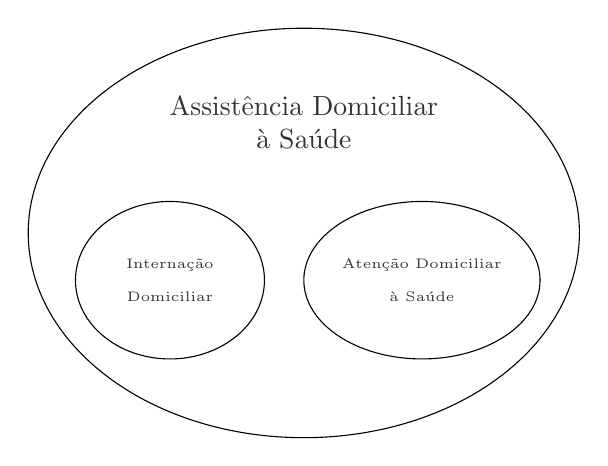
\begin{tikzpicture}
         \begin{scope}[shift={(0cm,0cm)}, fill opacity=0.8]
             \draw (0,0) ellipse (3.5cm and 2.6cm);
             \draw (-1.7,-0.6) ellipse (1.2cm and 1cm);
             \draw (1.5,-0.6) ellipse (1.5cm and 1cm);

             \node at (0,1.4) [align=center]{Assistência Domiciliar\\ à Saúde};
             \node at (-1.7,-0.6) [align=center]{\tiny Internação\\ \tiny Domiciliar};
             \node at (1.5,-0.6)[align=center]{\tiny Atenção Domiciliar\\ \tiny à Saúde};
             \end{scope}
         \end{tikzpicture} 
        \caption{}
        \label{fig:ads-categoria-tavoloari}
      \end{subfigure}
      ~
      \begin{subfigure}[b]{.45\textwidth}
        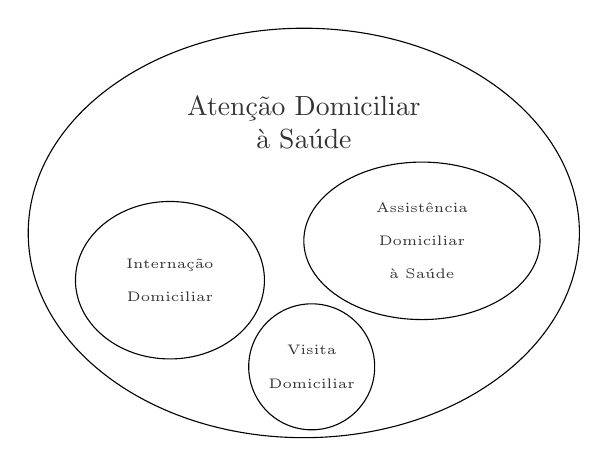
\begin{tikzpicture}
        \begin{scope}[shift={(0cm,0cm)}, fill opacity=0.8]
            \draw (0,0) ellipse (3.5cm and 2.6cm); % atencao domiciliar
            \draw (-1.7,-0.6) ellipse (1.2cm and 1cm); % internacao domiciliar
            \draw (1.5,-0.1) ellipse (1.5cm and 1cm); % assistencia domiciliar
            \draw (0.1, -1.7) circle (0.8cm); % visita domiciliar

            \node at (0,1.4) [align=center]{Atenção Domiciliar\\ à Saúde};
            \node at (-1.7,-0.6) [align=center]{\tiny Internação\\ \tiny Domiciliar};
            \node at (1.5,-0.1)[align=center]{\tiny Assistência\\ \tiny Domiciliar\\ \tiny à Saúde};
            \node at (0.1,-1.7)[align=center]{\tiny Visita\\ \tiny Domiciliar};
            \end{scope}
        \end{tikzpicture}
        \caption{}
        \label{fig:ads-categoria-giacamozzi}
      \end{subfigure}
      \par
      Fonte: Próprio autor.
    \end{center}
  \end{figure}